\documentclass[12pt, a4paper, oneside, openany, dvipsnames, hidelinks]{book}

  % Enables the use of colour. 
  \usepackage{xcolor}
  % Syntax high-lighting for code. Requires Python's pygments.
  \usepackage{minted}
  % Enables the use of umlauts and other accents.
  \usepackage[utf8]{inputenc}
  % Diagrams.
  \usepackage{tikz}
  % Settings for captions, such as sideways captions.
  \usepackage{caption}
  % Symbols for units, like degrees and ohms.
  \usepackage{gensymb}
  % Latin modern fonts - better looking than the defaults.
  \usepackage{lmodern}
  % Allows for columns spanning multiple rows in tables.
  \usepackage{multirow}
  % Better looking tables, including nicer borders.
  \usepackage{booktabs}
  % More math symbols.
  \usepackage{amssymb}
  % More math fonts, like mathbb.
  \usepackage{amsfonts}
  % More math layouts, equation arrays, etc.
  \usepackage{amsmath}
  % More theorem environments.
  \usepackage{amsthm}
  % More column formats for tables.
  \usepackage{array}
  % Adjust the sizes of box environments.
  \usepackage{adjustbox}
  % Better looking single quotes in verbatim and minted environments.
  \usepackage{upquote}
  % Better blank space decisions.
  \usepackage{xspace}
  % Better looking tikz trees.
  \usepackage{forest}
  % URLs.
  \usepackage{hyperref}
  % For plotting.
  \usepackage{pgfplots}
  % For filler.
  \usepackage{lipsum}
  
  % Various tikz libraries.
  % For drawing mind maps.
  \usetikzlibrary{mindmap}
  % For adding shadows.
  \usetikzlibrary{shadows}
  % Extra arrows tips.
  \usetikzlibrary{arrows.meta}
  % Old arrows.
  \usetikzlibrary{arrows}
  % Automata.
  \usetikzlibrary{automata}
  % For more positioning options.
  \usetikzlibrary{positioning}
  % Creating chains of nodes on a line.
  \usetikzlibrary{chains}
  % Fitting node to contain set of coordinates.
  \usetikzlibrary{fit}
  % Extra shapes for drawing.
  \usetikzlibrary{shapes}
  % For markings on paths.
  \usetikzlibrary{decorations.markings}
  % For advanced calculations.
  \usetikzlibrary{calc}
  
  % GMIT colours.
  \definecolor{gmitblue}{RGB}{20,134,225}
  \definecolor{gmitred}{RGB}{220,20,60}
  \definecolor{gmitgrey}{RGB}{67,67,67}
  
  % Tell minted to use the following colour scheme. 
  \usemintedstyle{manni}
  % Set some minted options.
  \setminted{frame=lines, framesep=2mm, baselinestretch=1.2, fontsize=\footnotesize, linenos}
  
  %% Change these:
  \newcommand{\thesistitle}{The Art of Computer Programming -- A difficult book to understand}
  \newcommand{\thesisauthor}{Ian McLoughlin}
  \newcommand{\thesisadvisor}{Dr Ian McLoughlin \\[1mm] Dr Ian McLoughlin \\[1mm] Dr Ian McLoughlin}
  \newcommand{\thesisdegree}{Master of Science}
  \newcommand{\thesisdate}{\today}
  \newcommand{\thesisinstitute}{Galway-Mayo Institute of Technology}
  \newcommand{\thesisdepartment}{Department of Computer Science and Applied Physics}
  %% End of things to change.

  % Begin the document.  
  \begin{document}
    % Include the titlepage  
    
%% Change these:
\newcommand{\thesistitle}{The Art of Computer Programming -- A difficult book to understand}
\newcommand{\thesisauthor}{Ian McLoughlin}
\newcommand{\thesisadvisor}{Dr Ian McLoughlin \\ Dr Ian McLoughlin \\ Dr Ian McLoughlin}
\newcommand{\thesisdegree}{Master of Science}
\newcommand{\thesisdate}{\today}
\newcommand{\thesisinstitute}{Galway-Mayo Institute of Technology}
\newcommand{\thesisdepartment}{Department of Computer Science and Applied Physics}
%% End of things to change.


% The title page.
\begin{titlingpage}
  
    % Display title.
  \begin{center}
    \begin{minipage}{\textwidth}
      \centering
      \rule{\linewidth}{0.2mm} \\[6mm]
      { \LARGE \bfseries \thesistitle } \\[2mm]
      \rule{\linewidth}{0.2mm}
    \end{minipage}
  \end{center}

  \vspace{16mm}

  % Display author.
  \begin{center}
    \begin{minipage}[t]{\textwidth}
      \centering
      {\small A thesis by} \\
      {\large \textbf{\thesisauthor}}
    \end{minipage}
  \end{center}

  \vspace{20mm}

  % Display degree.
  \begin{center}
    \begin{minipage}[t]{\textwidth}
      \centering
      {\small for the degree of} \\
      {\large \thesisdegree}
    \end{minipage}
  \end{center}
  
  \vspace{2mm}
  
  % Display advisors.
  \begin{center}
    \begin{minipage}[t]{\textwidth}
      \centering
      {\small advised by} \\
      \thesisadvisor
    \end{minipage}
  \end{center}

  \vspace{2mm}

  % Display date.
  \begin{center}
    \begin{minipage}[t]{\textwidth}
      \centering
      {\small submitted on} \\
      \thesisdate
    \end{minipage}
  \end{center}

  \vspace{2mm}

  % Display department.
  \begin{center}
    \begin{minipage}[t]{\textwidth}
      \centering
      {\small to the} \\
      \thesisdepartment \\
      \thesisinstitute
    \end{minipage}
  \end{center}

  \vspace{8mm}

  % Display institute.
  \begin{center}
    \begin{minipage}[t][30mm]{\textwidth}
      \centering
      
\includegraphics[width=80mm]{img/gmit-logo.jpg} \\[4mm]
    \end{minipage}
  \end{center}

\end{titlingpage}
    
    % Set the correct page number.
    \setcounter{page}{2}

    % Insert the table of contents.
    \tableofcontents

    % Include the chapter.
    %!TEX root = ../thesis.tex

\chapter*{About this project}
\paragraph{Abstract}
A brief description of the results.

\paragraph{Author}
Explain here who the author is.
    %!TEX root = ../thesis.tex

\chapter{Introduction}
\label{section:introduction}

In the introduction, you should describe what your thesis is about, how the
thesis is organised, and what the reader can expect as they read down through
it.
The most important aspect of the introduction is to set the context for the
rest of the thesis.
You should sign-post for the reader the most important parts of your work and
where they appear in the document.
In \LaTeX, you should refer to sections, tables, and figures using commands
rather than specifying a page or saying ``the table below''. The \texttt{ref}
command will keep track of changes to the layout to the document. So, for
example, I can just refer to Section \ref{section:literature} rather than
worrying where that might move to in future.
Note to refer to an item in the bibliography, you use the \texttt{cite} command,
which should generally be placed after a \texttt{tilde}(\texttt{\~}) rather than
a space~\cite{einstein}.


\section{Sections}

The introduction chapter of a Ph.D. thesis serves as the gateway to your research and sets the stage for the reader to understand the context, significance, and objectives of your study. Here's a comprehensive guide on what to include in the introduction chapter:

Background and Context:

Provide an overview of the broader field of study and the specific research area your thesis addresses. Discuss the historical background, key concepts, theories, and previous research relevant to your topic.
Research Problem and Motivation:

Clearly articulate the research problem or question your thesis aims to address. Explain why this problem is significant and worthy of investigation. Discuss any gaps or limitations in existing literature that your research seeks to fill.
Objectives and Research Questions:

State the objectives of your research and the specific research questions you seek to answer. These objectives should be clear, specific, and aligned with the overall purpose of your study.
Scope and Limitations:

Define the scope of your research by outlining what is included and excluded from your study. Discuss any limitations or constraints that may impact the interpretation or generalizability of your findings.
Conceptual Framework or Theoretical Framework:

If applicable, introduce the conceptual framework or theoretical framework that underpins your research. Explain the theoretical perspectives, models, or frameworks you will use to guide your analysis and interpretation.
Methodology:

Provide an overview of the research methodology and approach you have adopted. Discuss the research design, data collection methods, analytical techniques, and any other procedures used to conduct your study.
Significance and Contributions:

Clearly articulate the significance of your research and the potential contributions it makes to the field. Explain how your study advances knowledge, addresses gaps in the literature, or has practical implications.
Organizational Structure:

Outline the structure of your thesis by briefly describing the contents of each chapter. Provide a roadmap that helps the reader navigate through your thesis and understand the sequence of your argumentation.
Literature Review:

While the main literature review may be presented in a separate chapter, briefly summarize the key literature that informs your research in the introduction. Highlight the most relevant theories, concepts, and empirical studies that provide context for your study.
Engage the Reader:

Write in a clear, engaging, and concise manner to capture the reader's interest. Use compelling language and examples to draw the reader into the topic and motivate them to continue reading.
Remember, the introduction chapter sets the tone for your entire thesis and should provide a comprehensive overview of your research topic, objectives, methodology, and significance. It should be well-structured, focused, and persuasive, laying the foundation for the reader to understand and appreciate the rest of your work.

\subsection{Subsections}
You might even use subsections if you really need to.
There are also subsubsections in \LaTeX, but be careful not to overdo it.

\lipsum[1-2]

\subsection{Maxwell's Equations}

\subsubsection{Gauss's Law for Electricity}
Gauss's Law for Electricity is one of the four fundamental equations in classical electromagnetism, formulated by Carl Friedrich Gauss.
It describes the relationship between the electric flux through a closed surface and the electric charge enclosed within that surface.
Mathematically, Gauss's Law for Electricity is expressed as:
\[
\oint_S \mathbf{E} \cdot d\mathbf{A} = \frac{Q_{\text{enc}}}{\varepsilon_0}
\]
Here's an explanation of the key components of Gauss's Law for Electricity:
\begin{itemize}
  \item $\oint_S$ represents a closed surface integral over a closed surface $S$. This means that we are summing the electric field ($\mathbf{E}$) over all infinitesimal areas ($d\mathbf{A}$) of the closed surface $S$.
  
  \item $\mathbf{E}$ is the electric field vector at each point on the surface. It represents the force experienced by a unit positive charge placed at that point.
  
  \item $d\mathbf{A}$ is a vector representing an infinitesimal area element of the surface. It is oriented perpendicular to the surface at each point.
  
  \item $Q_{\text{enc}}$ is the total electric charge enclosed within the closed surface $S$. This includes the sum of all positive and negative charges within the enclosed region.
  
  \item $\varepsilon_0$ is the permittivity of free space, a fundamental constant in electromagnetism. It represents the ability of a material to permit the formation of an electric field in response to an applied electric field.
\end{itemize}

In simpler terms, Gauss's Law for Electricity states that the total electric flux through a closed surface is proportional to the total electric charge enclosed within that surface, with the constant of proportionality being the permittivity of free space.
In other words, it quantifies how much electric field passes through a closed surface due to the presence of electric charges inside that surface.


\subsubsection{Gauss's Law for Magnetism}
Gauss's Law for Magnetism states that the magnetic flux through any closed surface is always zero.
Mathematically, it is expressed as:
\[
\oint_S \mathbf{B} \cdot d\mathbf{A} = 0
\]
Here's an explanation of the key components of Gauss's Law for Magnetism:
\begin{itemize}
  \item $\oint_S$ represents a closed surface integral over a closed surface $S$. This means that we are summing the magnetic field ($\mathbf{B}$) over all infinitesimal areas ($d\mathbf{A}$) of the closed surface $S$.
  
  \item $\mathbf{B}$ is the magnetic field vector at each point on the surface. Unlike electric fields, magnetic fields do not have sources or sinks (monopoles), so the magnetic flux through any closed surface is always zero.
  
  \item $d\mathbf{A}$ is a vector representing an infinitesimal area element of the surface. It is oriented perpendicular to the surface at each point.
\end{itemize}

In summary, Gauss's Law for Magnetism implies that there are no magnetic monopoles (isolated north or south poles), and the magnetic flux through any closed surface is always zero, indicating that magnetic field lines neither start nor end but always form closed loops.


\subsubsection{Faraday's Law of Induction}
Faraday's Law of Induction describes how a changing magnetic field induces an electromotive force (EMF) and hence an electric current in a conducting loop.
Mathematically, it is expressed as:
\[
\oint_C \mathbf{E} \cdot d\boldsymbol{\ell} = -\frac{d\Phi_B}{dt}
\]
Here's an explanation of the key components of Faraday's Law of Induction:
\begin{itemize}
  \item $\oint_C$ represents a closed path integral around a closed loop $C$. This means that we are summing the electric field ($\mathbf{E}$) around the closed loop $C$.
  
  \item $\mathbf{E}$ is the induced electric field within the conducting loop. It is created by a changing magnetic flux through the loop according to Faraday's law.
  
  \item $d\boldsymbol{\ell}$ is a vector representing an infinitesimal displacement along the closed loop $C$.
  
  \item $d\Phi_B/dt$ represents the rate of change of magnetic flux ($\Phi_B$) through the surface enclosed by the loop with respect to time. The negative sign indicates that the induced EMF and hence the induced electric field opposes the change in magnetic flux.
\end{itemize}

In summary, Faraday's Law of Induction states that a changing magnetic field induces an electric field and hence an electromotive force (EMF) in any closed conducting loop, producing an electric current in the loop. This phenomenon forms the basis of many practical devices, such as electric generators and transformers.


\subsubsection{Ampere's Circuital Law (with Maxwell's addition)}

Amp\`ere's Circuital Law relates the magnetic field around a closed loop to the electric current passing through the loop. With Maxwell's addition, it accounts for the displacement current, which arises from changing electric fields. Mathematically, it is expressed as:

\[
\oint_C \mathbf{B} \cdot d\boldsymbol{\ell} = \mu_0 \left( I_{\text{enc}} + \varepsilon_0 \frac{d\Phi_E}{dt} \right)
\]

Here's an explanation of the key components of Amp\`ere's Circuital Law (with Maxwell's addition):

\begin{itemize}
  \item $\oint_C$ represents a closed path integral around a closed loop $C$. This means that we are summing the magnetic field ($\mathbf{B}$) around the closed loop $C$.
  
  \item $\mathbf{B}$ is the magnetic field vector at each point along the closed loop $C$.
  
  \item $d\boldsymbol{\ell}$ is a vector representing an infinitesimal displacement along the closed loop $C$.
  
  \item $\mu_0$ is the permeability of free space, a fundamental constant in electromagnetism.
  
  \item $I_{\text{enc}}$ is the total current passing through the loop $C$. This includes both conduction current and displacement current.
  
  \item $\varepsilon_0$ is the permittivity of free space, another fundamental constant in electromagnetism.
  
  \item $\frac{d\Phi_E}{dt}$ represents the rate of change of electric flux ($\Phi_E$) through the surface enclosed by the loop with respect to time. This gives rise to the displacement current, which is included in Amp\`ere's law with Maxwell's addition.
\end{itemize}

In summary, Amp\`ere's Circuital Law with Maxwell's addition states that the magnetic field around a closed loop is proportional to the total current passing through the loop, including both conduction current and displacement current arising from changing electric fields. This law plays a crucial role in understanding the behavior of electromagnetic fields in various physical systems.


    \chapter{Literature}
\label{section:literature}

One of the most important parts of a thesis is an overview of work done by
others.
This gives the reader confidence that you are speaking from a knowledgable
position, that you have done your hoemwork on the subject.
You should not just list out a bunch of papers you have found in journals.
Rather, you need to find the most relevant papers, describe their main results
and how they relate to your work, and also give a brief critique of the work if
necessary.


\section{Sources}

Look at the beautiful mathematics in this equation:
\begin{equation}
  \label{eq:euler}
  e^{i\pi} + 1 = 0
\end{equation}
It belongs to Euler, and is often cited as an example of the beauty of mathematics.

The sources of information you use are important too.
You'll need to use the academic literature, but you'll also likely need to use
technical specifications and other non-academic sources of literature.
They should all be referenced.
See the \texttt{bibliography.bib} file for information about referencing.

\lipsum[16-25]



    \chapter{Methodology}
Check out the nice graphs in Figure \ref{tikz:graphs}.

\lipsum[26]

\begin{figure}[ht]
  \centering
  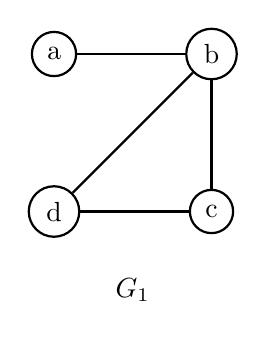
\begin{tikzpicture}
    \begin{scope}[every node/.style={circle,thick,draw}]
      \node (a) at (0,2) {a};
      \node (b) at (2,2) {b};
      \node (c) at (2,0) {c};
      \node (d) at (0,0) {d};
    \end{scope}
    \begin{scope}[every edge/.style={draw=black,thick}]
      \path (a) edge (b);
      \path (b) edge (c);
      \path (b) edge (d);
      \path (c) edge (d);
    \end{scope}
    \node () at (1,-1) {$G_1$};
  \end{tikzpicture}
  \hspace{1.5cm}
  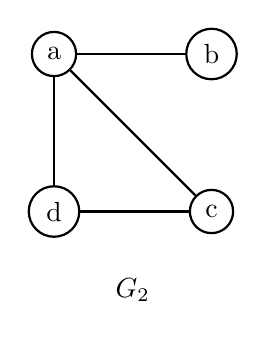
\begin{tikzpicture}
    \begin{scope}[every node/.style={circle,thick,draw}]
      \node (1) at (0,2) {a};
      \node (2) at (2,2) {b};
      \node (3) at (2,0) {c};
      \node (4) at (0,0) {d};
    \end{scope}
    \begin{scope}[every edge/.style={draw=black,thick}]
      \path (1) edge (2);
      \path (1) edge (3);
      \path (1) edge (4);
      \path (3) edge (4);
    \end{scope}
    \node () at (1,-1) {$G_2$};
  \end{tikzpicture}
  \caption{Nice pictures}
  \label{tikz:graphs}
\end{figure}

\lipsum[26-28]
    \chapter{Prototype code}
Look at my nice program in Listing \ref{code:tuesday}.

\begin{listing}[ht]
  \begin{minted}{python}
# Ian McLoughlin, 2018-02-01
# Is it Tuesday?

import datetime

if datetime.datetime.today().weekday() == 1:
  print("Yay! It is Tuesday.")
else:
  print("Unfortunately it is not Tuesday.")
  \end{minted}
  \caption{Is it Tuesday?}
  \label{code:tuesday}
\end{listing}

    \chapter{Something interesting}
You will sometimes, over the course of your research, find something
particularly interesting. If you think it is worthy of a published paper in
its own right, you can add a chapter about it.

\lipsum[25]

Table \ref{table:mytable} is a nice table.

\lipsum[30]

\begin{figure}[h]
  \centering
  \begin{tabular}{cc}
    \toprule
    Column 1 & Column 2 \\
    \midrule
    Hello & world! \\
    \bottomrule
  \end{tabular}
  \caption{A table.}
  \label{table:mytable}
\end{figure}


\lipsum[20-25]
    \chapter{Conclusion}
The conclusion generally summaries the thesis and suggest further work you
would like to complete based on the work in your thesis.

\lipsum[20-30]

    % Include the bibliography with IEEE style.
    \bibliographystyle{ieeetr}
    \bibliography{bibliography}
  \end{document}
